\chapter{Methodology} \label{sec:methodology}

\section{Multi Fidelity Modeling} \label{sec:mf_modeling}

Tools of varying complexity, accuracy, and cost are often used for analyses of engineering designs. Combining data from these tools has several benefits. The cost of analysis can be lowered by performing high-fidelity simulations only in areas where the uncertainty in lower-fidelity simulations is high. Additionally, surrogate models built using multi-fidelity data require significantly fewer computationally-expensive high-fidelity evaluations to accurately model trends in the data \cite{robinson2008surrogate}. Finally, the combination of predictions obtained with analysis tools of varying levels of fidelity (in the prediction of the QoIs and their associated uncertainties) opens up the possibility for the use of multi-fidelity information fusion methods that can be significantly more accurate than any of the individual predictions alone.

\subsection{Gaussian Process Regression}\label{sec:GPR}
The basic building block of our multi-fidelity framework is Gaussian Process (GP) regression \cite{rasmussen_gaussian_2006}, which is a supervised learning technique used to build a surrogate model for an unknown function $y = f(\mathbf{x})$ given $n$ observed input-output pairs $\mathcal{D} = \{\mathbf{x}_i, y_i\}$ for $i \in\{1,...,n\}$. The function can be non-deterministic and have noise, $\sigma$, associated with its observations. In the context of this work, the computer simulations are deterministic but have modeling errors that are treated as noise in the function of interest. The unknown function can have multi-dimensional inputs, but must have a scalar output. These input-output pairs can be arranged in matrices $X$ and $\mathbf{y}$. If the function has an $m$ dimensional input then $X$ is an $\left (n \times m \right)$ matrix of inputs and $\mathbf{y}$ is an $\left (n \times 1 \right)$ vector of outputs.

Since these observations can be imperfect, each observation is assumed to carry some Gaussian noise associated with it such that $y_i \sim \mathcal{N}(E(f(\mathbf{x_i})),\sigma_i^2)$. Assuming that all the observations in $\mathcal{D}$ have a joint Gaussian distribution, a GP can be used as a surrogate model for the data. A GP is completely defined by its mean function, $ \mu(\mathbf{x}) $, and a kernel function, $\mathbf{k}(\mathbf{x,x';\theta})$, that is parameterized by some hyperparameters $\theta$. For the purposes of this study, the squared exponential function is used as the kernel function: 
\begin{equation}
    \mathbf{k}\left (\mathbf{x,x'} \right ) = \sigma_f^2 \exp \left ( -\sum_{d=1}^{d=m}\frac{\left ( x_d - x'_d \right )^2}{2l_d} \right ),
\end{equation}
where $m$ is the dimension of the input. The hyperparameters for this kernel function are the signal variance $\sigma_f^2$ and the length scales $l_d$. The kernel function is used to create a kernel matrix $K \in \mathbb{R} ^{ n \times n}$ where $K_{ij} = \mathbf{k \left( x_i, x_j \right )}$.

To enable the GP to estimate functions with a non-zero mean, the mean of $f(\mathbf{x})$ is represented using $p$ fixed basis functions, $\mathbf{h(x)}$, and learned regression coefficients $\beta$. At a minimum, these basis functions include a constant term, but can have multiple polynomial terms. With these in mind, the surrogate model $Z$ evaluated at some location of interest, $\mathbf{x}_*$, can be represented as some mean value plus a zero-mean GP: 
\begin{equation}
    Z(\mathbf{x}_*) = \mathbf{h(\mathbf{x}_*)}^T\beta + \mathcal{GP}(0,K(\mathbf{x}_*,\mathbf{x}_*';\theta)).
\end{equation}
The $n_*$ sample locations and the basis functions can also be arranged in matrices $X_* \in \mathbb{R} ^{ n_* \times m}$ and $H \in \mathbb{R} ^{ p \times n_*}$ such that each row of $X_*$ is a $m$-dimensional sample location and each column of $H_*$ is a $p$-dimensional result of the basis functions at the locations in $X_*$.

Combining the GP regression equations for noisy observations with those incorporating explicit basis functions, and writing in the matrix notation, the surrogate model is defined as 
\begin{equation}
    Z(X_*) \sim \mathcal{GP} (\mu(X_*), \sigma^2(X_*,X_*)),
\end{equation}
\begin{equation} \label{equ:mu_gpr}
    \mu(X_*) = H_*^T\hat{\beta} + K(X_*,X)[K(X,X)+\text{diag}(\sigma_i)]^{-1} (y-H^T\hat{\beta}), 
\end{equation}
\begin{equation} \label{equ:sig_gpr}
    \sigma^2(X_*,X_*) = K(X_*,X_*) - K(X_*,X)[K(X,X)+\text{diag}(\sigma_i)]^{-1} K(X,X_*), 
\end{equation}
where $\hat{\beta} = (H^TV^{-1}H)^{-1}H^TV^{-1}y$ is the best linear estimator for the basis coefficients and $V = K(X,X) + \text{diag}(\sigma_i)$ represents the kernel matrix at the observed points $\left ( K(X,X) \right )$ and includes the Gaussian noise that is associated with each observation $\left ( \sigma_i \right )$. The prediction from the surrogate model $Z(X_*)$ is defined by the mean $\mu(X_*)$ and the uncertainty associated with these predictions is represented by the diagonal of the $\sigma^2(X_*,X_*)$ function. To fully define the GP, the hyperparameters of the kernel function need to be learned from the data. The hyperparameters are chosen by maximizing the marginal log-likelihood of the model, 

\begin{equation}
    \log~p(y|x;\theta) = -\frac{1}{2} \log|V| - \frac{1}{2}\alpha^T V^{-1}\alpha - \frac{n}{2}\log 2\pi,
\end{equation}
where $\alpha = \left ( y-H^T\hat{\beta} \right )$.

\subsection{Recursive Formulation for Multi-Fidelity Gaussian Processes}\label{sec:MF_GP}
It is often the case that simulations or experiments of a sufficiently-high fidelity are too expensive to perform over the entire domain of interest for a modeled problem. In many cases, there are lower-fidelity approximations available that can be evaluated quickly to perform parameter studies. The aim of the multi-fidelity GP is to use data from different fidelity levels to create a surrogate model that can best approximate the highest-fidelity function and its uncertainty, while reducing the required number of high-fidelity function evaluations. 

Assume there are $s$ information sources $f_t(\mathbf{x})$, where $t\in\{1,2,...,s\}$, and the function at the highest fidelity level, $f_s(\mathbf{x})$, is being approximated using a Gaussian Processes, $Z_s(\mathbf{x}) \sim \mathcal{N}(\mu_{s}(\mathbf{x}), \sigma_s^2(\mathbf{x}))$. An auto-regressive formulation of the multi-fidelity framework is used. This was first put forward in \cite{kennedy_predicting_2000} and was improved upon by \cite{gratiet_multi-fidelity_nodate} to reduce computational cost and improve predictions. The GP approximation at the $t$ fidelity level is modeled as

\begin{equation}
    Z_t(\mathbf{x}) = \rho_{t-1}(\mathbf{x})Z_{t-1}(\mathbf{x}) + \delta_t(\mathbf{x}),
\end{equation}
\begin{equation}
    \rho_{t-1}(\mathbf{x}) = \mathbf{g}_{t-1}^T(\mathbf{x})\beta_{\rho_{t-1}},
\end{equation}
where $\mathbf{g}_{t-1}(\mathbf{x})$ is a set of $q$ basis functions, similar to $\mathbf{h}(\mathbf{x})$ in the previous section, $\beta_{\rho_{t-1}}$ is the learned regression coefficients, and $\delta_t(\mathbf{x})$ is modeled using a GP. A way to interpret these terms is to consider $\delta_t(\mathbf{x})$ the additive bias and $\rho_{t-1}(\mathbf{x})$ the multiplicative bias between fidelity levels $t$ and $t-1$. To account for the different fidelity levels and their corresponding data, the subscript $t$ is added to the notation introduced in Section \ref{sec:GPR}. For example, $X_t$ refers to all the input data at level $t$. Additionally, the term $\Sigma_t = \text{diag}(\sigma^2_{i,t})$ is introduced, which refers to the noise in the outputs $\mathbf{y_t}$. 

In Appendix B of \cite{gratiet_multi-fidelity_nodate}, Gratiet presents the predictive equations for the case when the design sets are not nested ($\mathcal{D}_t \notin \mathcal{D}_{t-1}$) and the data has no process noise, such that $\Sigma_t$ is a null matrix. This work extends those equations to include process noise $\Sigma_t \neq \emptyset$, which produces the following representations for the mean and covariance equations for fidelity level $t \neq 1$ as

\begin{equation}\label{equ:mu_Zt}
\begin{split}
    \mu_{t}(X_*) = & ~ \rho_{t-1} \left ( X_* \right ) \mu_{t-1} \left (X_* \right ) + H_*^T\beta_t + \\
    & \left [ \left ( \rho_{t-1} \left (X_* \right ) \rho_{t-1} \left (X_t \right )^T \right ) \odot \sigma^2_{t-1} \left(X_*,X_t \right) + K_{t} \left(X_*,X_t \right)\right] \\ 
    & \left [ \left ( \rho_{t-1} \left (X_t \right ) \rho_{t-1} \left (X_t \right )^T \right ) \odot \sigma^2_{t-1} \left(X_t,X_t \right) + V_t \right ]^{-1} \\ 
    & \left (\mathbf{y}_t - \rho_{t-1} \left (X_t \right ) \odot \mu_{t-1} \left (X_t \right) - F_t^T \beta_t \right),
\end{split}
\end{equation}
and
\begin{equation}\label{equ:sig_Zt}
\begin{split}
    \sigma^2_{t}(X, \Tilde{X}) = & ~ \left (\rho_{t-1} \left ( X \right ) \rho_{t-1} ( \Tilde{X})^T \right ) \odot \sigma^2_{t-1} (X, \Tilde{X}) + K_t(X, \Tilde{X}) - \\
    & \left [ \left ( \rho_{t-1} \left (X \right ) \rho_{t-1} \left (X_t \right )^T \right ) \odot \sigma^2_{t-1} \left(X,X_t \right) + K_{t} \left(X,X_t \right)\right] \\ 
    & \left [ \left ( \rho_{t-1} \left (X_t \right ) \rho_{t-1} \left (X_t \right )^T \right ) \odot \sigma^2_{t-1} \left(X_t,X_t \right) + V_t \right ]^{-1} \\ 
    & \left [ \left ( \rho_{t-1} \left (X_t \right ) \rho_{t-1} ( \Tilde{X} )^T \right ) \odot \sigma^2_{t-1} (X_t, \Tilde{X} ) + K_{t} ( X_t, \Tilde{X} ) \right], 
\end{split}
\end{equation}
where $(X, \Tilde{X})$ are generic input arguments, $V_t = K_{t} \left(X_t,X_t \right) + \Sigma_t $, and $\rho_{t-1} (X) = G_{t-1}(X)^T \beta_{\rho_{t-1}}$. $G_{t-1}(X)$ is a $q \times n$ matrix where each column is a $q$-dimensional result of the basis functions for the corresponding $m$-dimensional row of input samples in $X$, and $\beta_{\rho_{t-1}}$ are learned regression coefficients. For the lowest fidelity level, $t=1$, the regular GP regression equations, Equations (\ref{equ:mu_gpr}, \ref{equ:sig_gpr}) are used. For a set of sample locations $X_*$, the mean predictions at fidelity level $t$ is given by $\mu_t(X_*)$ and the variance in the predictions is given by the diagonal of $\sigma^2_t(X_*,X_*)$. 

To fully define the GP of each fidelity level, the regression coefficients ($\beta_{\rho_{t-1}}$ and $\beta_t$) and the hyperparameters of the kernel functions of each fidelity level need to be learned from the data. The parameter estimation equations from  \cite{gratiet_multi-fidelity_nodate} are extended for noisy observations:

\begin{equation}
    \begin{bmatrix}
    \beta_t & \beta_{\rho_{t-1}}
    \end{bmatrix} = \left [ J_t^T \left ( K_t(X_t,X_t) + \Sigma_t \right )^{-1} J_t \right ]^{-1} \left [ J_t^T \left ( K_t(X_t,X_t) + \Sigma_t \right ) ^{-1} \mathbf{y_t} \right ], 
\end{equation}
with $J_1 = H_1$ and for $t > 1$, $J_t =  \begin{bmatrix} G_{t-1} \odot \left ( \mu_{t-1} \left ( X_t \right )  \mathbf{1}_{q_{t-1}} \right ) & F_t \end{bmatrix}$. $\mathbf{1}_{q_{t-1}} \in \mathbb{R} ^{q_{t-1} \times n_t} $ is a matrix of ones. The hyperparameters of the kernel functions are learned by minimizing the negative marginal log-likelihood of each fidelity level.

\begin{equation}
    \log~p(\mathbf{y}_t|X;\theta) = -\left (\frac{1}{2} \log|V_t| + \frac{1}{2} \alpha^T V_t^{-1} \alpha + \frac{n_t}{2}\log 2\pi \right),
\end{equation}
where $\alpha = \left (\mathbf{y_t} - \rho_{t-1} \beta_{\rho_{t-1}}-F_t\beta_t \right )$.

As mentioned earlier in this section, the recursive formulation put forth by Gratiet \cite{le_gratiet_recursive_2014} improves on the work originally done by Kennedy and O'Hagan \cite{kennedy_predicting_2000} by reducing the computational complexity of the training and sampling steps of the multi-fidelity GP. This is achieved by splitting the dataset into each individual fidelity level instead of agglomerating the data from all levels into one set of equations. This results in having to invert smaller matrices, which greatly improves the computational cost of the process. Figure \ref{fig:time_comp} shows the comparative times for the training and sampling steps. Two simple one-dimensional, analytic functions were used to generate the result: 

\begin{equation}
    f_1(x) = 0.5 \left ( 6x - 2\right )^2 \sin{ \left (12x -4 \right )} + 10 \left ( x - 0.5 \right ) -5 ~\text{and}
\end{equation}
\begin{equation}
        f_2(x) = 2f_1(x) - 20x + 20.
\end{equation}
where $f_2(x)$ is the high-fidelity function that is approximated by a lower fidelity function, $f_1(x)$.
In this case, the number of high-fidelity data points ($n_2$) and low-fidelity data points ($n_1$) had a constant ratio: $\frac{n_2}{n_1} = 0.2$. These savings in computational time increase with more fidelity levels and higher-dimensional functions. 

\begin{figure}
    \centering
    \begin{subfigure}[Time taken to train the multi-fidelity GP.] {
        \includegraphics[width=.45\textwidth]{images/time_process.eps} }
    \end{subfigure}
    \hfill
    \begin{subfigure}[Time taken to sample the multi-fidelity GP.]{
        \includegraphics[width=.45\textwidth]{images/time_query.eps} 
    }
    \end{subfigure}
    \caption{Wall clock time comparison to train and query the multi-fidelity Gaussian Process formulations put forth by Kennedy and O'Hagan \cite{kennedy_predicting_2000}, and Gratiet \cite{gratiet_multi-fidelity_nodate}. \label{fig:time_comp}}
\end{figure}

\section{Reynolds-Averaged Navier-Stokes (RANS) UQ Methodology overview}\label{sec:rans_uq}

Computational Fluid Dynamics (CFD) is widely used in industry to predict turbulent fluid flows of engineering interest. Turbulent flows are characterized by irregular, small-scale fluctuations in the flow variables (velocity, density, pressure) that make the fluid flow chaotic and computationally intractable to simulate exactly. While higher-fidelity approaches such as large-eddy simulations (LES) and direct numerical simulations (DNS) exist, their prohibitively-large computational cost limits their adoption in industrial design workflows today. 

Instead, relatively inexpensive RANS simulations with turbulence models are most commonly used to describe turbulent flows for engineering applications. Reynolds averaging starts with the decomposition of the chaotic velocity field ($ u_i$) into its mean ($\overline{u_i}$) and fluctuating ($u_i'$) velocity components such that $u_i = \overline{u_i} + u_i'$. Here $i$ denotes a coordinate direction, $i=1, 2, 3$. This allows for the ensemble-averaging of the Navier-Stokes equations \cite{pope_2000} which leads to a closure problem due to the resulting non-linear $\overline{u_i'u_j'}$ term that has to be modeled. This term is also known as the Reynolds stress tensor, $R_{ij}$. 

Turbulence models are concerned with predicting the behavior of the Reynolds stress tensor throughout a flow of interest (and without specific data about that particular flow) in a computationally tractable manner. To this end, these models often make simplifying assumptions about the tensor that can inject significant uncertainties into their predictions. For example, a popular assumption that is employed in numerous turbulence models is the Boussinesq approximation (also known as the linear eddy viscosity hypothesis). It assumes that $R_{ij}$ can be defined by a combination of the mean rate of strain ($S_{ij}$), an eddy viscosity ($\nu_t$), and the turbulent kinetic energy ($k$):
 
 \begin{equation}
     R_{ij} = \nu_t S_{ij} - \frac{2}{3} k \delta_{ij},
 \end{equation}
where $S_{ij} = \left ( \frac{\partial \overline{u_i}}{\partial x_j} + \frac{\partial \overline{u_j}}{\partial x_i} \right )$, $x_i$ is a coordinate direction and $\delta_{ij}$ is the Kronecker delta. This linear eddy viscosity model purports a simplified proportional relationship between the Reynolds stress tensor and the mean rate of strain tensor. It assumes that the turbulent fluid is an isotropic medium where the direction of Reynolds stresses are always aligned with the mean strain rate. Although reasonable for simple flows without adverse pressure gradients, this assumption can severely limit the flow features that can be predicted by the turbulence model, thus introducing uncertainty into the QoIs predicted by RANS simulations. The shortcomings of the Boussinesq assumption are particularly evident in areas of the operating envelope of an aircraft where separated flows and shock-boundary layer interactions exist. 

To better understand the effects of such an assumption, the eigenspace perturbation methodology was developed by Mishra, Iaccarino, and Ghili \cite{iaccarino_eig_pert}. It aims to quantify model-form uncertainties that arise from the use of turbulence models in RANS simulations by introducing perturbations in the eigenvalues and eigenvectors of the Reynolds stress anisotropy tensors $\left ( b_{ij} \right )$ that are predicted by the models. The methodology was recently validated for aerospace problems of interest and implemented in the open-source SU2 solver by Mishra et al. \cite{mishra_uncertainty_2019}.  This methodology does not rely on any higher-fidelity data. To explain the perturbations that are introduced, the stress tensor is decomposed into its anisotropic and deviatoric components as
 
\begin{equation}
    R_{ij}=2k(b_{ij}+\frac{\delta_{ij}}{3}).
\end{equation}
Here, $k~(=\frac{R_{ii}}{2})$ is the turbulent kinetic energy and $b_{ij}$ is the Reynolds stress anisotropy tensor. The anisotropy tensor can be further decomposed into its eigenvalues and eigenvectors and represented as

\begin{equation}\label{equ:eigendecomposition}
b_{ij}=Q \Lambda Q^T,
\end{equation}
where $\Lambda$ is a diagonal matrix that contains the eigenvalues $\lambda_i \in \mathbb{R}$ \cite{Gerolymos2016AlgebraicPA}, and $Q$ is a matrix where the $i$-th column represents the eigenvector corresponding to $\lambda_i$. The matrices $Q$ and $\Lambda$ are ordered such that $\lambda_{1}\geq\lambda_{2}\geq\lambda_{3}$. To understand the eigenspace perturbations it helps to visualize the Reynolds stress tensor as an ellipsoid, where the axes of the ellipsoid are defined by the eigenvectors, the relative lengths along each of the axes are defined by the corresponding eigenvalues, and the size of the ellipsoid is defined by the turbulent kinetic energy. An example of such an ellipsoid, represented in a coordinate system defined by the eigenvectors of $S_{ij}$, is shown in Figure \ref{fig:pert_vis} \textbf{(d)}. 

The perturbations are designed to exercise the limits of the physical realizability constraints placed on the Reynolds stress tensor \cite{schumann1977realizability,speziale1994realizability,2014realizability}. One way to graphically represent the constraints placed on the anisotropic part of the stress tensor is to use the eigenvalues ($\Lambda$) to project the stress tensor onto an anisotropy-invariant map, which often takes the form of a triangle. The vertices of the triangle represent the one-, two- and three-component limiting states of turbulence (referred to as the $1C$, $2C$, and $3C$ states) and all of the physically realizable states of the stress tensor lie within the triangle. One such representation of an anisotropy-invariant map is the barycentric map \cite{banerjee2007presentation}. This mapping allows the writing of the projection as a convex combination of the limiting states of turbulence: 

\begin{equation}
    \textbf{x} = \textbf{x}_{1C} (\lambda_1 - \lambda_2) + \textbf{x}_{2C} (2\lambda_2 - 2\lambda_3) + \textbf{x}_{3C} (3\lambda_3 + 1), 
\end{equation}
where $\textbf{x}_{1C}$, $\textbf{x}_{2C}$, and $\textbf{x}_{3C}$ are the coordinates of the vertices that represent the one-, two-, and three-component limiting states of turbulence. For example, the stress ellipsoid shown in Figure \ref{fig:pert_vis} \textbf{(d)} would be mapped on to the barycentric map as shown in Figure \ref{fig:pert_vis} \textbf{(a)}.

The eigenvalue perturbations are performed such that the limiting states of turbulence are simulated. This involves perturbing the state of the tensor, sequentially, to each of the vertices of the triangle. The eigenvalues resulting from these perturbations are: 

\begin{equation}\label{equ:eigenvalue_pert}
    \Lambda^*_{1C} = 
    \begin{bmatrix}
    2/3 & 0    & 0 \\
    0   & -1/3 & 0 \\
    0   & 0    & -1/3
    \end{bmatrix},~
    \Lambda^*_{2C} = 
    \begin{bmatrix}
    1/6 & 0   & 0 \\
    0   & 1/6 & 0 \\
    0   & 0   & -1/3
    \end{bmatrix},~
    \Lambda^*_{3C} = 
    \begin{bmatrix}
    0 & 0 & 0 \\
    0 & 0 & 0 \\
    0 & 0 & 0
    \end{bmatrix}.
\end{equation}
where $*$ represents the perturbed state. The eigenvector perturbation involves changing the alignment such that the perturbed state is
\begin{equation}\label{equ:eigenvector_pert}
    Q^* = Qv
\end{equation}
where $v$ is either:
\begin{equation}\label{equ:vmin_vmax}
    v_{max} = 
    \begin{bmatrix}
    1 & 0 & 0 \\
    0 & 1 & 0 \\
    0 & 0 & 1
    \end{bmatrix},~
    v_{min} = 
    \begin{bmatrix}
    0 & 0 & 1 \\
    0 & 1 & 0 \\
    1 & 0 & 0
    \end{bmatrix}.
\end{equation}
Combining the eigendecomposition from Equation \eqref{equ:eigendecomposition}, the eigenvalue perturbations from Equation \eqref{equ:eigenvalue_pert}, and the eigenvector perturbations from Equations (\ref{equ:eigenvector_pert}, \ref{equ:vmin_vmax}), the perturbed anisotropy tensor can be built as
\begin{equation}
    b^*_{ij}=Q^* \Lambda^* Q^{*T}.
\end{equation}

In the case shown in Figure \ref{fig:pert_vis} \textbf{(b)}, the eigenvalues are perturbed to the 1C limiting state. This corresponds to changing the shape of the ellipsoid to be infinitely long in one direction, as shown in Figure \ref{fig:pert_vis} \textbf{(e)}. Consequently, the eigenvector alignment is changed to maximize turbulent kinetic energy production ($v_{max}$). This is represented in Figure \ref{fig:pert_vis} \textbf{(c)} and \textbf{(f)}. The change in alignment of the eigenvector can not be represented in the barycentric map, which is why Figures \ref{fig:pert_vis} \textbf{(c)} and \textbf{(b)} are identical.

\begin{figure}
    \center
    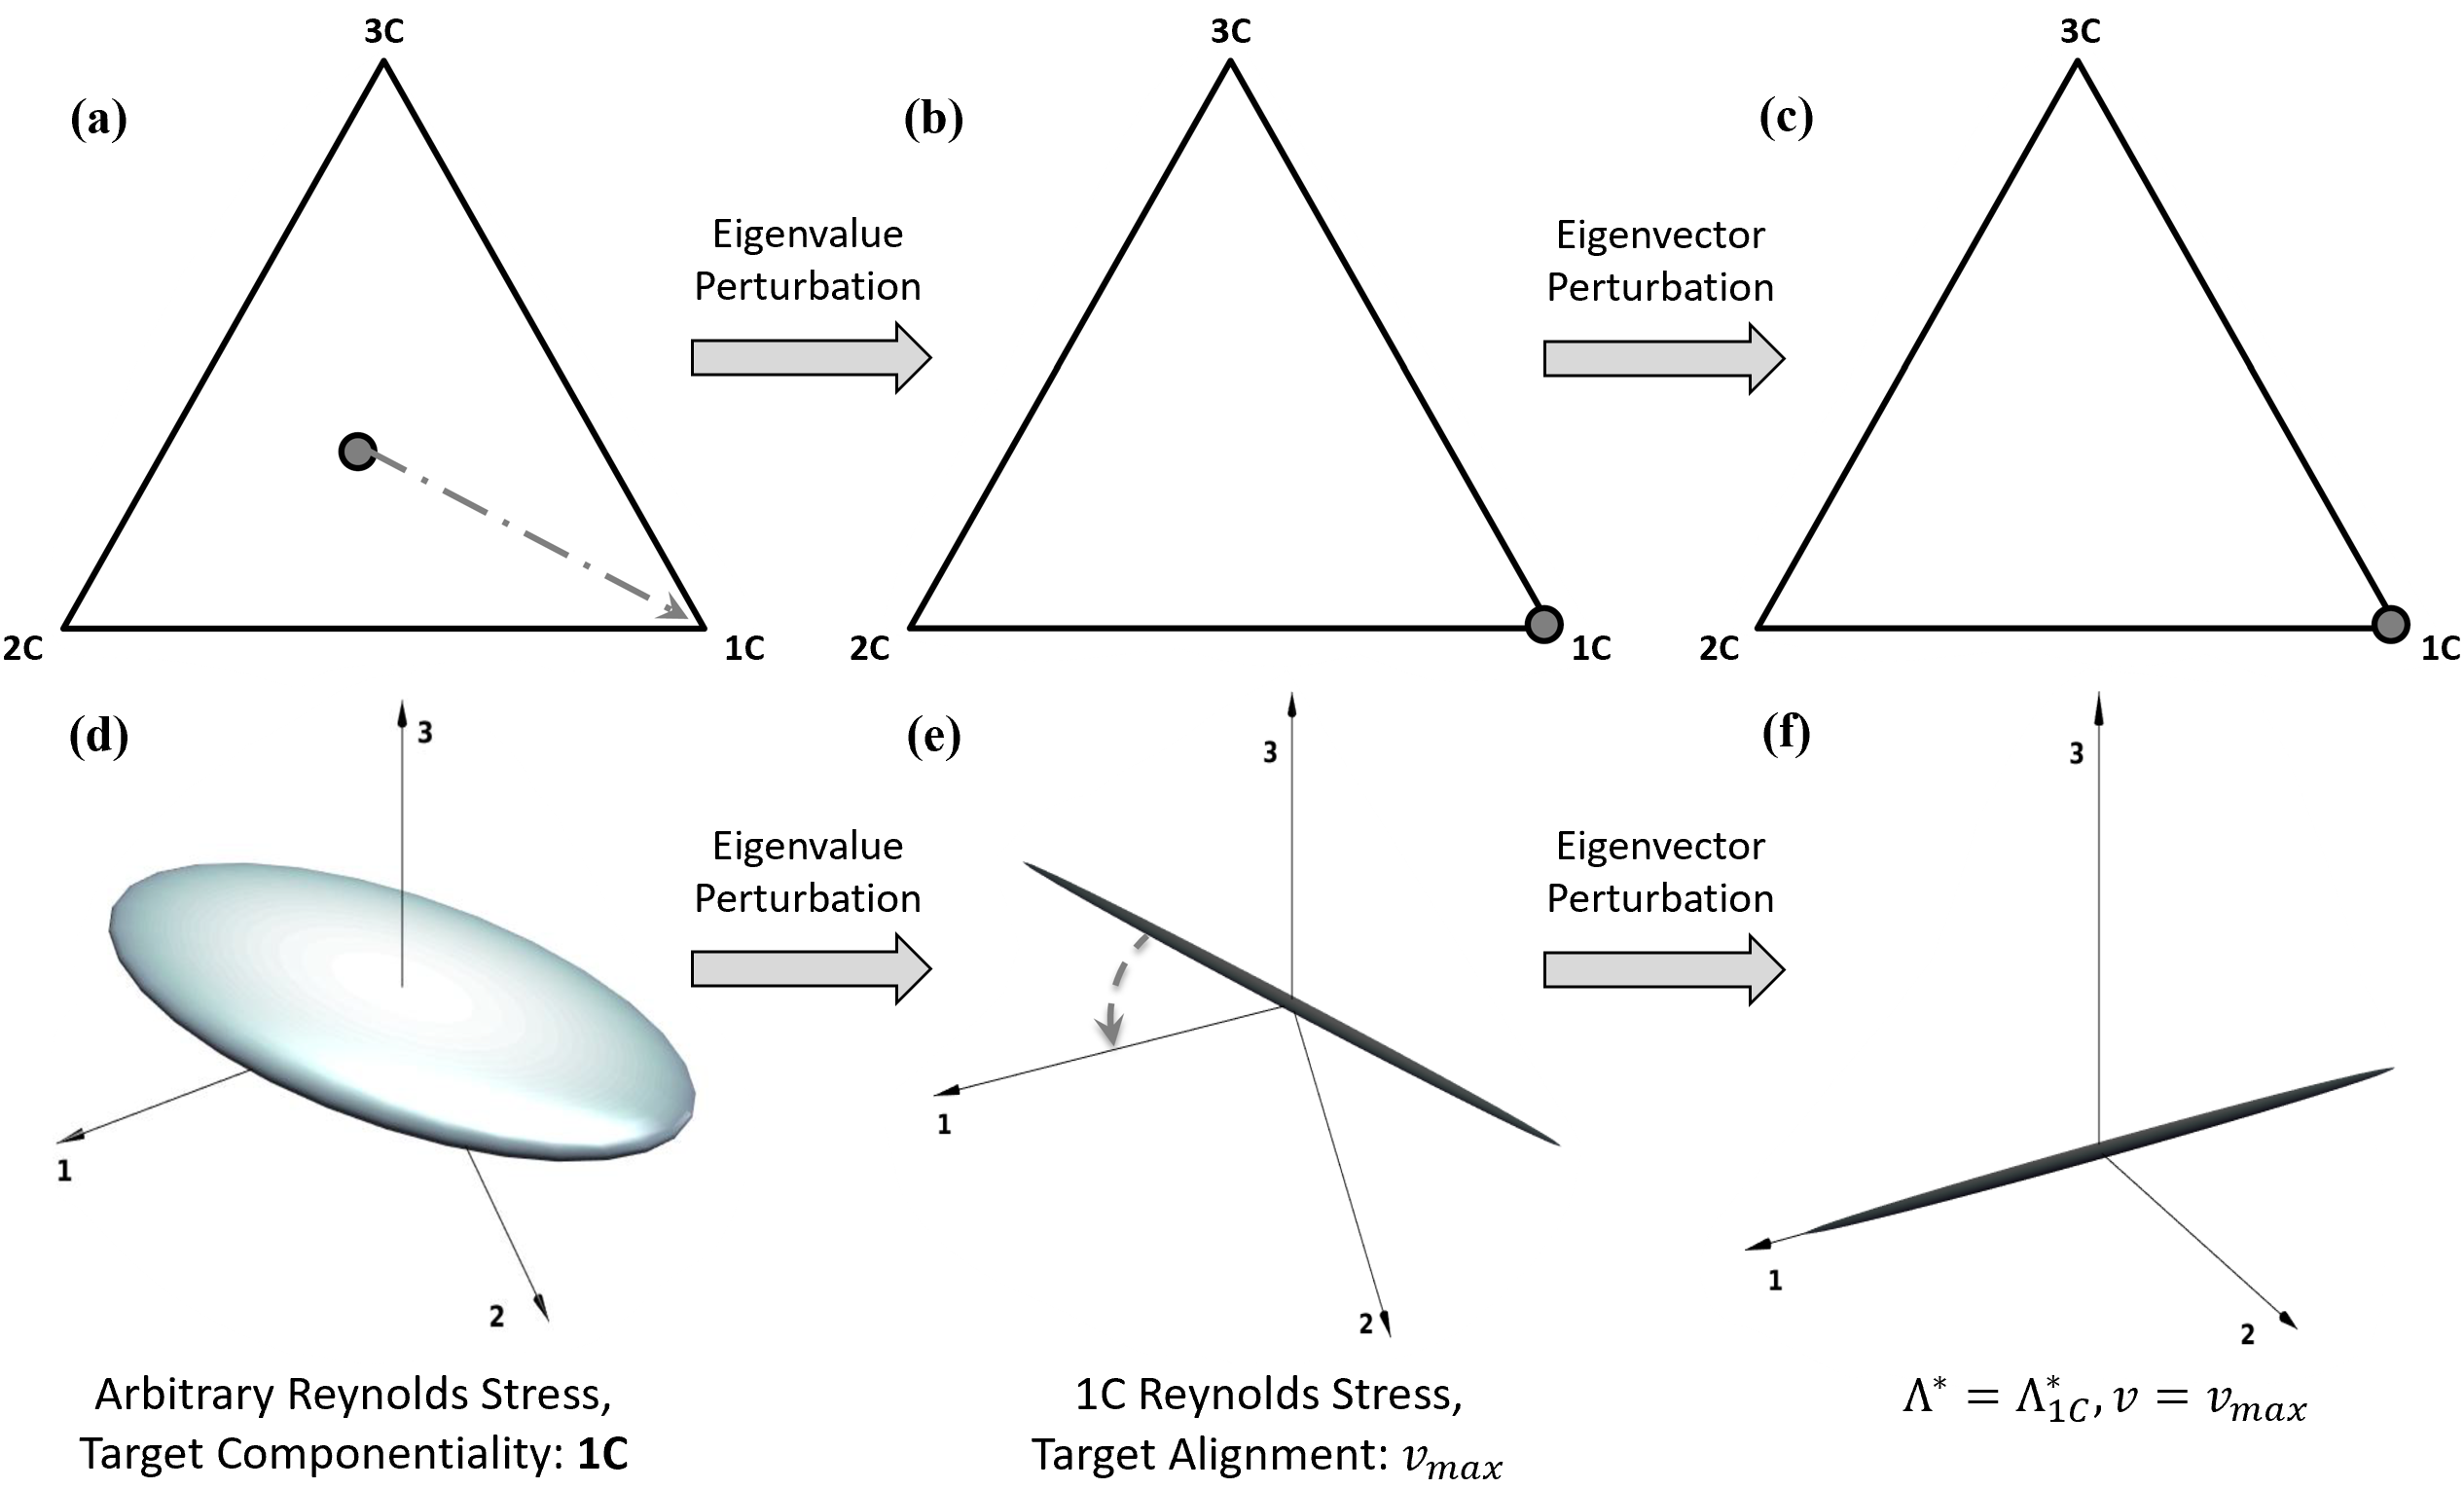
\includegraphics[width=0.95\textwidth]{images/eig_pert_1c.png}
    \caption{Schematic outline of Eigenspace perturbations from an arbitrary state of the Reynolds stress. \label{fig:pert_vis}}
\end{figure}

The combinations of 3 eigenvalue perturbations (towards the $1C, 2C$, and $3C$ states) and 2 eigenvector perturbations ($v_{min}$ and $v_{max}$) result in 5 unique sets of perturbations. The resulting Reynolds stress ellipsoid shapes are shown in Figure \ref{fig:all_perts}. This number of perturbations is 5, and not 6, because the $3C$ eigenvalue perturbation results in a rotationally symmetric stress ellipsoid, which means the eigenvector perturbation doesn't change anything. These 5 perturbed states correspondingly require 5 different RANS simulations, in addition to the baseline simulation with the unmodified version of the turbulence model, to provide information about the uncertainty introduced by the turbulence model. For each simulation, the same perturbation is applied uniformly across the entire computational domain. This uniform perturbation is a non-physical assumption. Research is ongoing in leveraging higher-fidelity simulations (LES, DNS) to infer correlations between different parts of the computational domain and the perturbation that should be applied. For the purpose of this work, each perturbation is carried out uniformly everywhere, at each pseudo-time step, and the simulation is run to convergence. This results in 5 new realizations of the flow field in addition to the flow field predicted by the unperturbed turbulence model. The maximum and minimum values of any QoI predicted by these 6 (5 perturbed + 1 baseline) simulations create the interval bound for that QoI. These interval bounds are then used in the multi-fidelity framework as uncertainty estimates for CFD simulations. Note that the additional 5 simulations for the perturbed turbulence model can be run simultaneously and, if sufficient computational resources are available, the entire process of RANS UQ can be completed in the same wall-clock time as a typical deterministic RANS simulation.

An inherent assumption is that the maximum and minimum value of any QoI occurs at the corners of the barycentric triangle, and not somewhere in the interior. In \cite{emory2014visualizing} the bounds were shown to be monotonically increasing as the perturbation magnitude increases. This means that the interval bound is largest at the corner when perturbing along that direction. It is still possible that there could be a different direction of perturbation that would result in larger interval bounds. For example, the largest interval could result from a perturbation towards one of the sides of the barycentric triangle. To exercise the limits of the componentiality of the turbulence field, the perturbations occur towards each vertex of the triangle. 

The theoretical underpinnings of the eigenspace perturbation methodology have been discussed in detail by Mishra and Iaccarino \cite{mishra_perturbations_2019}. They prove that the eigenspace perturbations extend the isotropic eddy viscosity assumption to an anisotropic relation between the mean velocity gradients and the Reynolds stresses. This represents the most general relationship between the mean gradients and the Reynolds stresses, $ R_{ij}=\nu_{ijkl}S_{kl}+\mu_{ijkl}W_{kl}$, where $S_{kl}$ and $W_{kl}$ represent the mean rates of strain and rotation respectively. This extension enables the perturbed models to account for the effects of flow separation, secondary flows, highly anisotropic flows, etc. 

The eigenspace perturbation methodology has exhibited substantial success in a variety of engineering applications. This methodology has been successfully applied to the analysis of uncertainty in flows through scramjets \cite{emory2011characterizing}, contoured aircraft nozzles \cite{aiaajets, envelopingmodels}, and turbomachinery designs \cite{emory2016uncertainty}. The methodology has been used for the design optimization under uncertainty of turbine cascades \cite{razaaly2019optimization}. In civil engineering applications, this methodology has been applied in the design of urban canopies \cite{garcia2014quantifying,ricci2015local}. Owing to the structural similarity between the RANS and LES paradigms, this methodology has been extended and successfully applied for the uncertainty estimation of Large Eddy Simulations and scalar flux models \cite{gorle2013framework} as well.

\begin{figure}
    \centering
    \begin{subfigure}[$2C$ state with $v_{max}$ eigenvector alignment.] {
        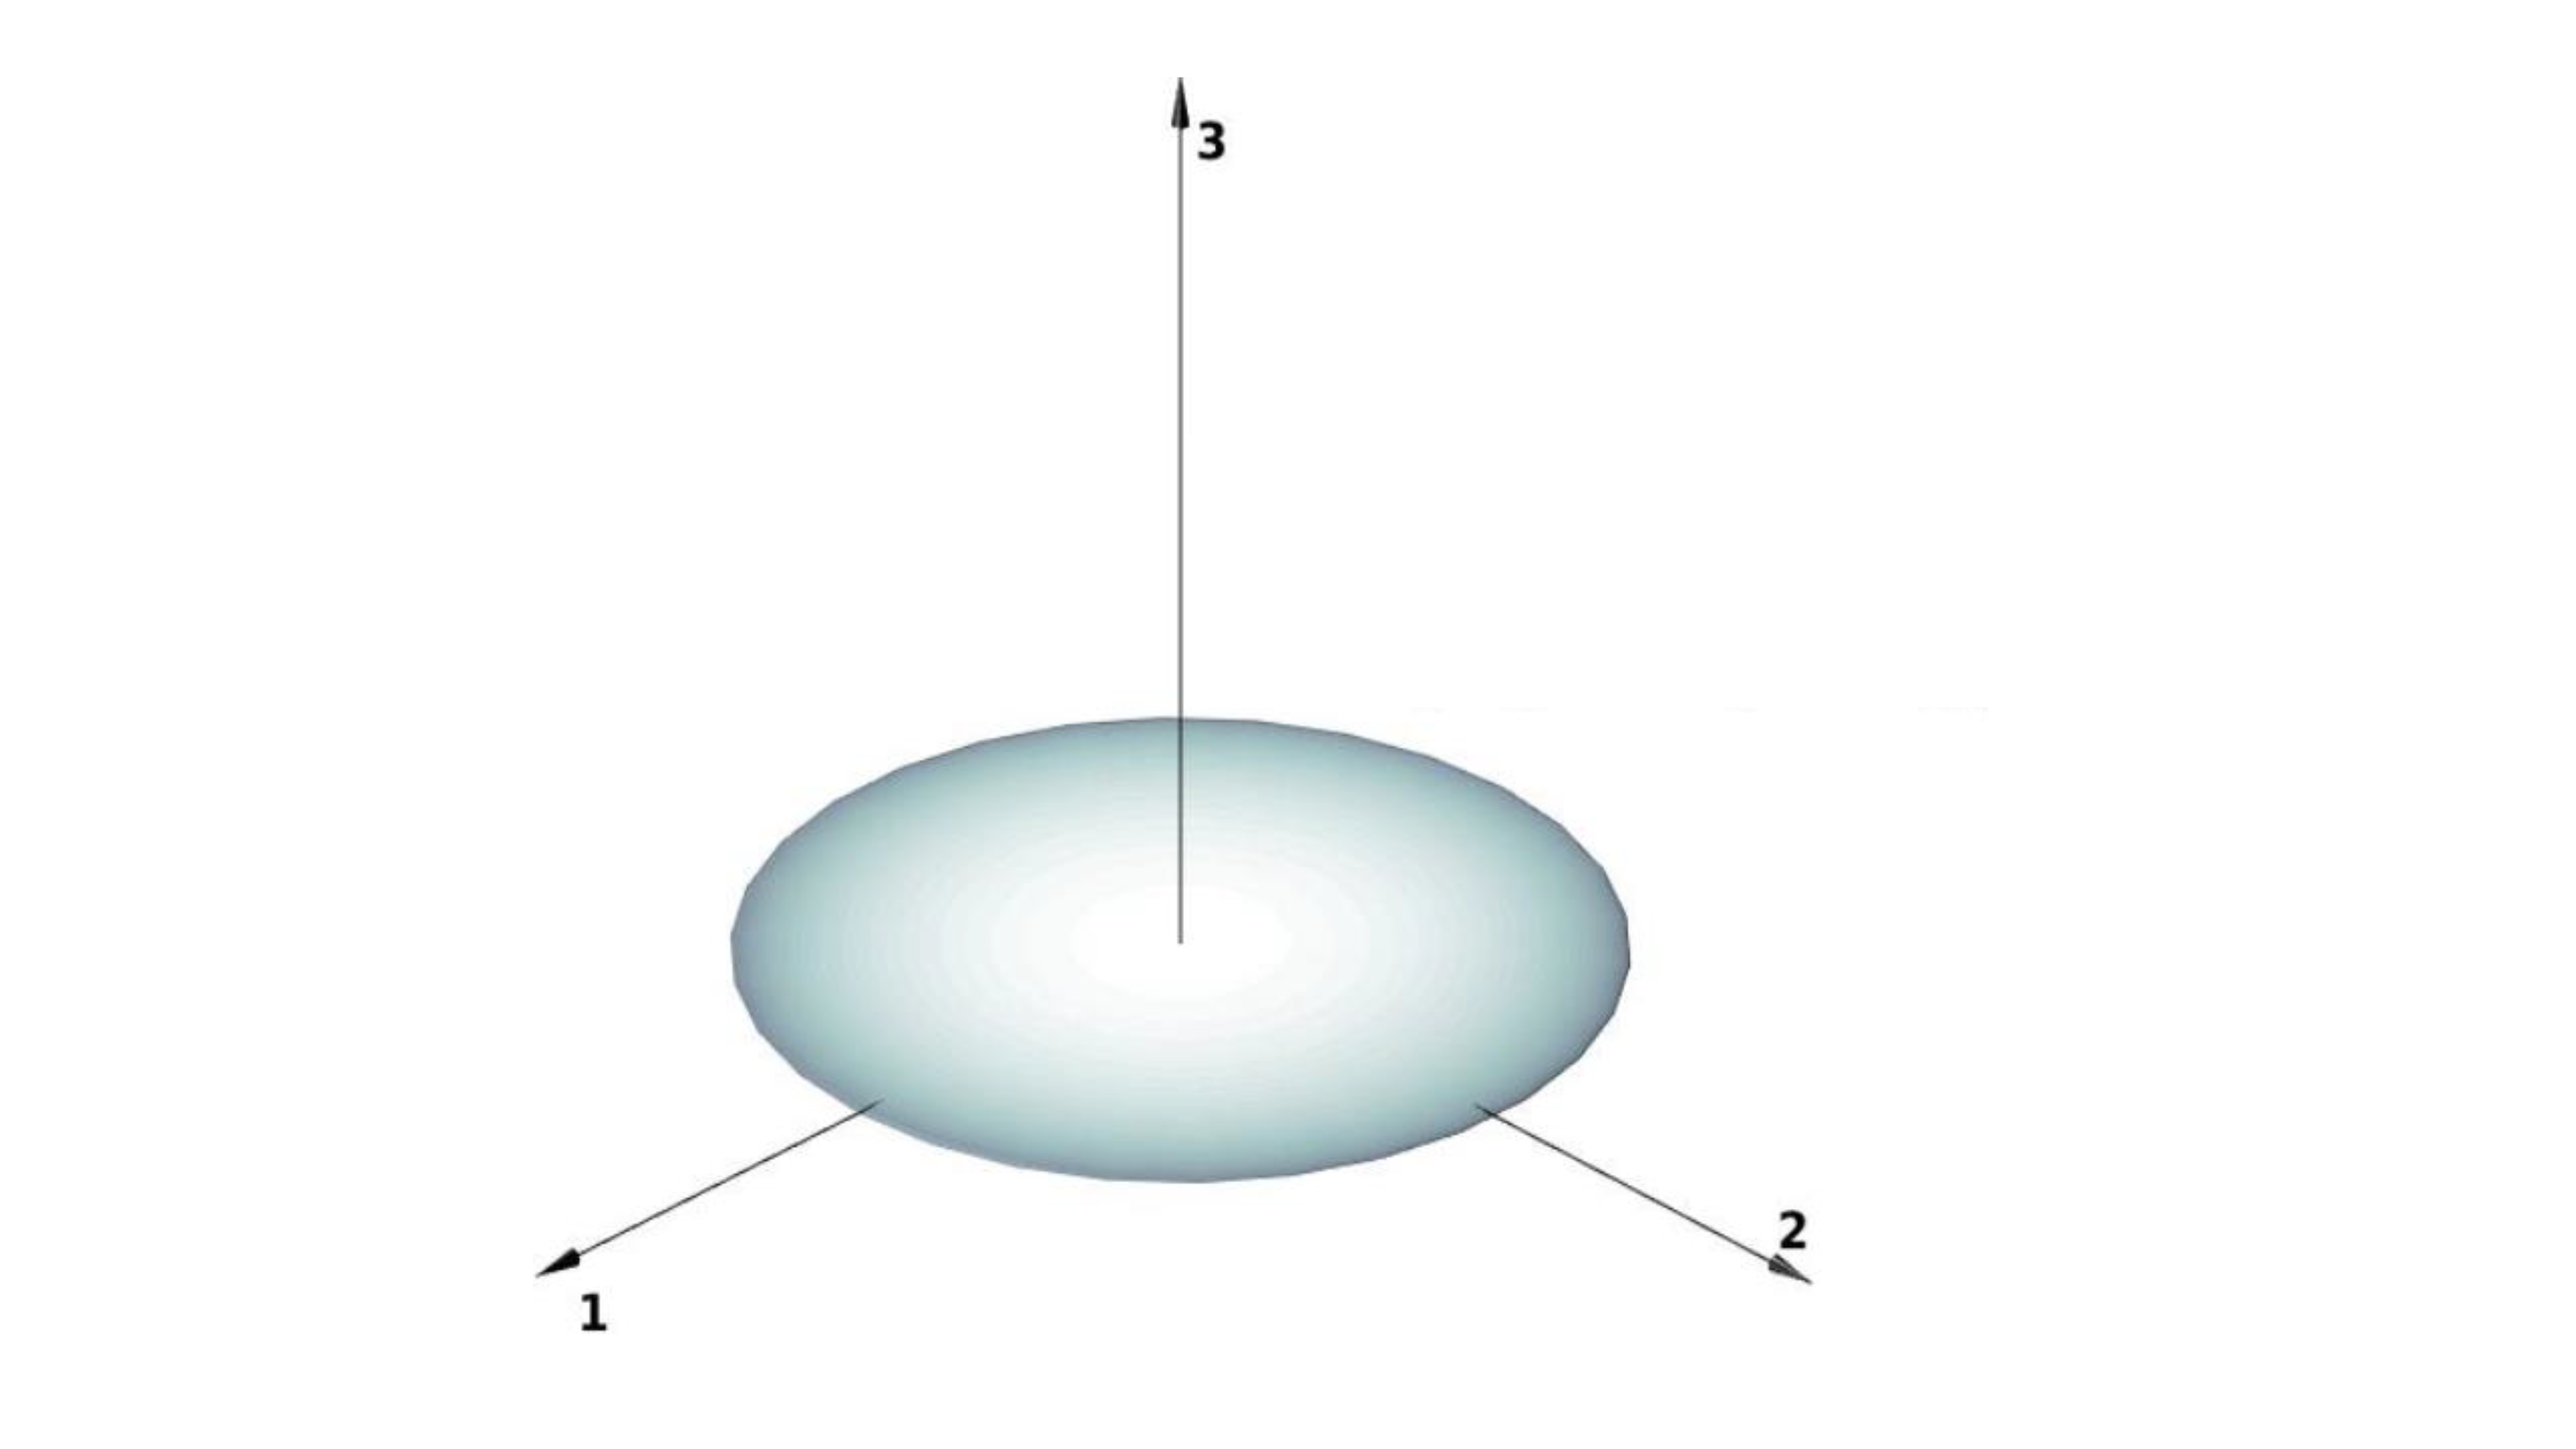
\includegraphics[trim=200 40 280 30, clip,             width=000.24\textwidth]{images/2c_max.png}
        \label{fig:2c_max}
    }
    \end{subfigure}
    \hspace{10pt}
    \begin{subfigure}[$2C$ state with $v_{min}$ eigenvector alignment.]{
        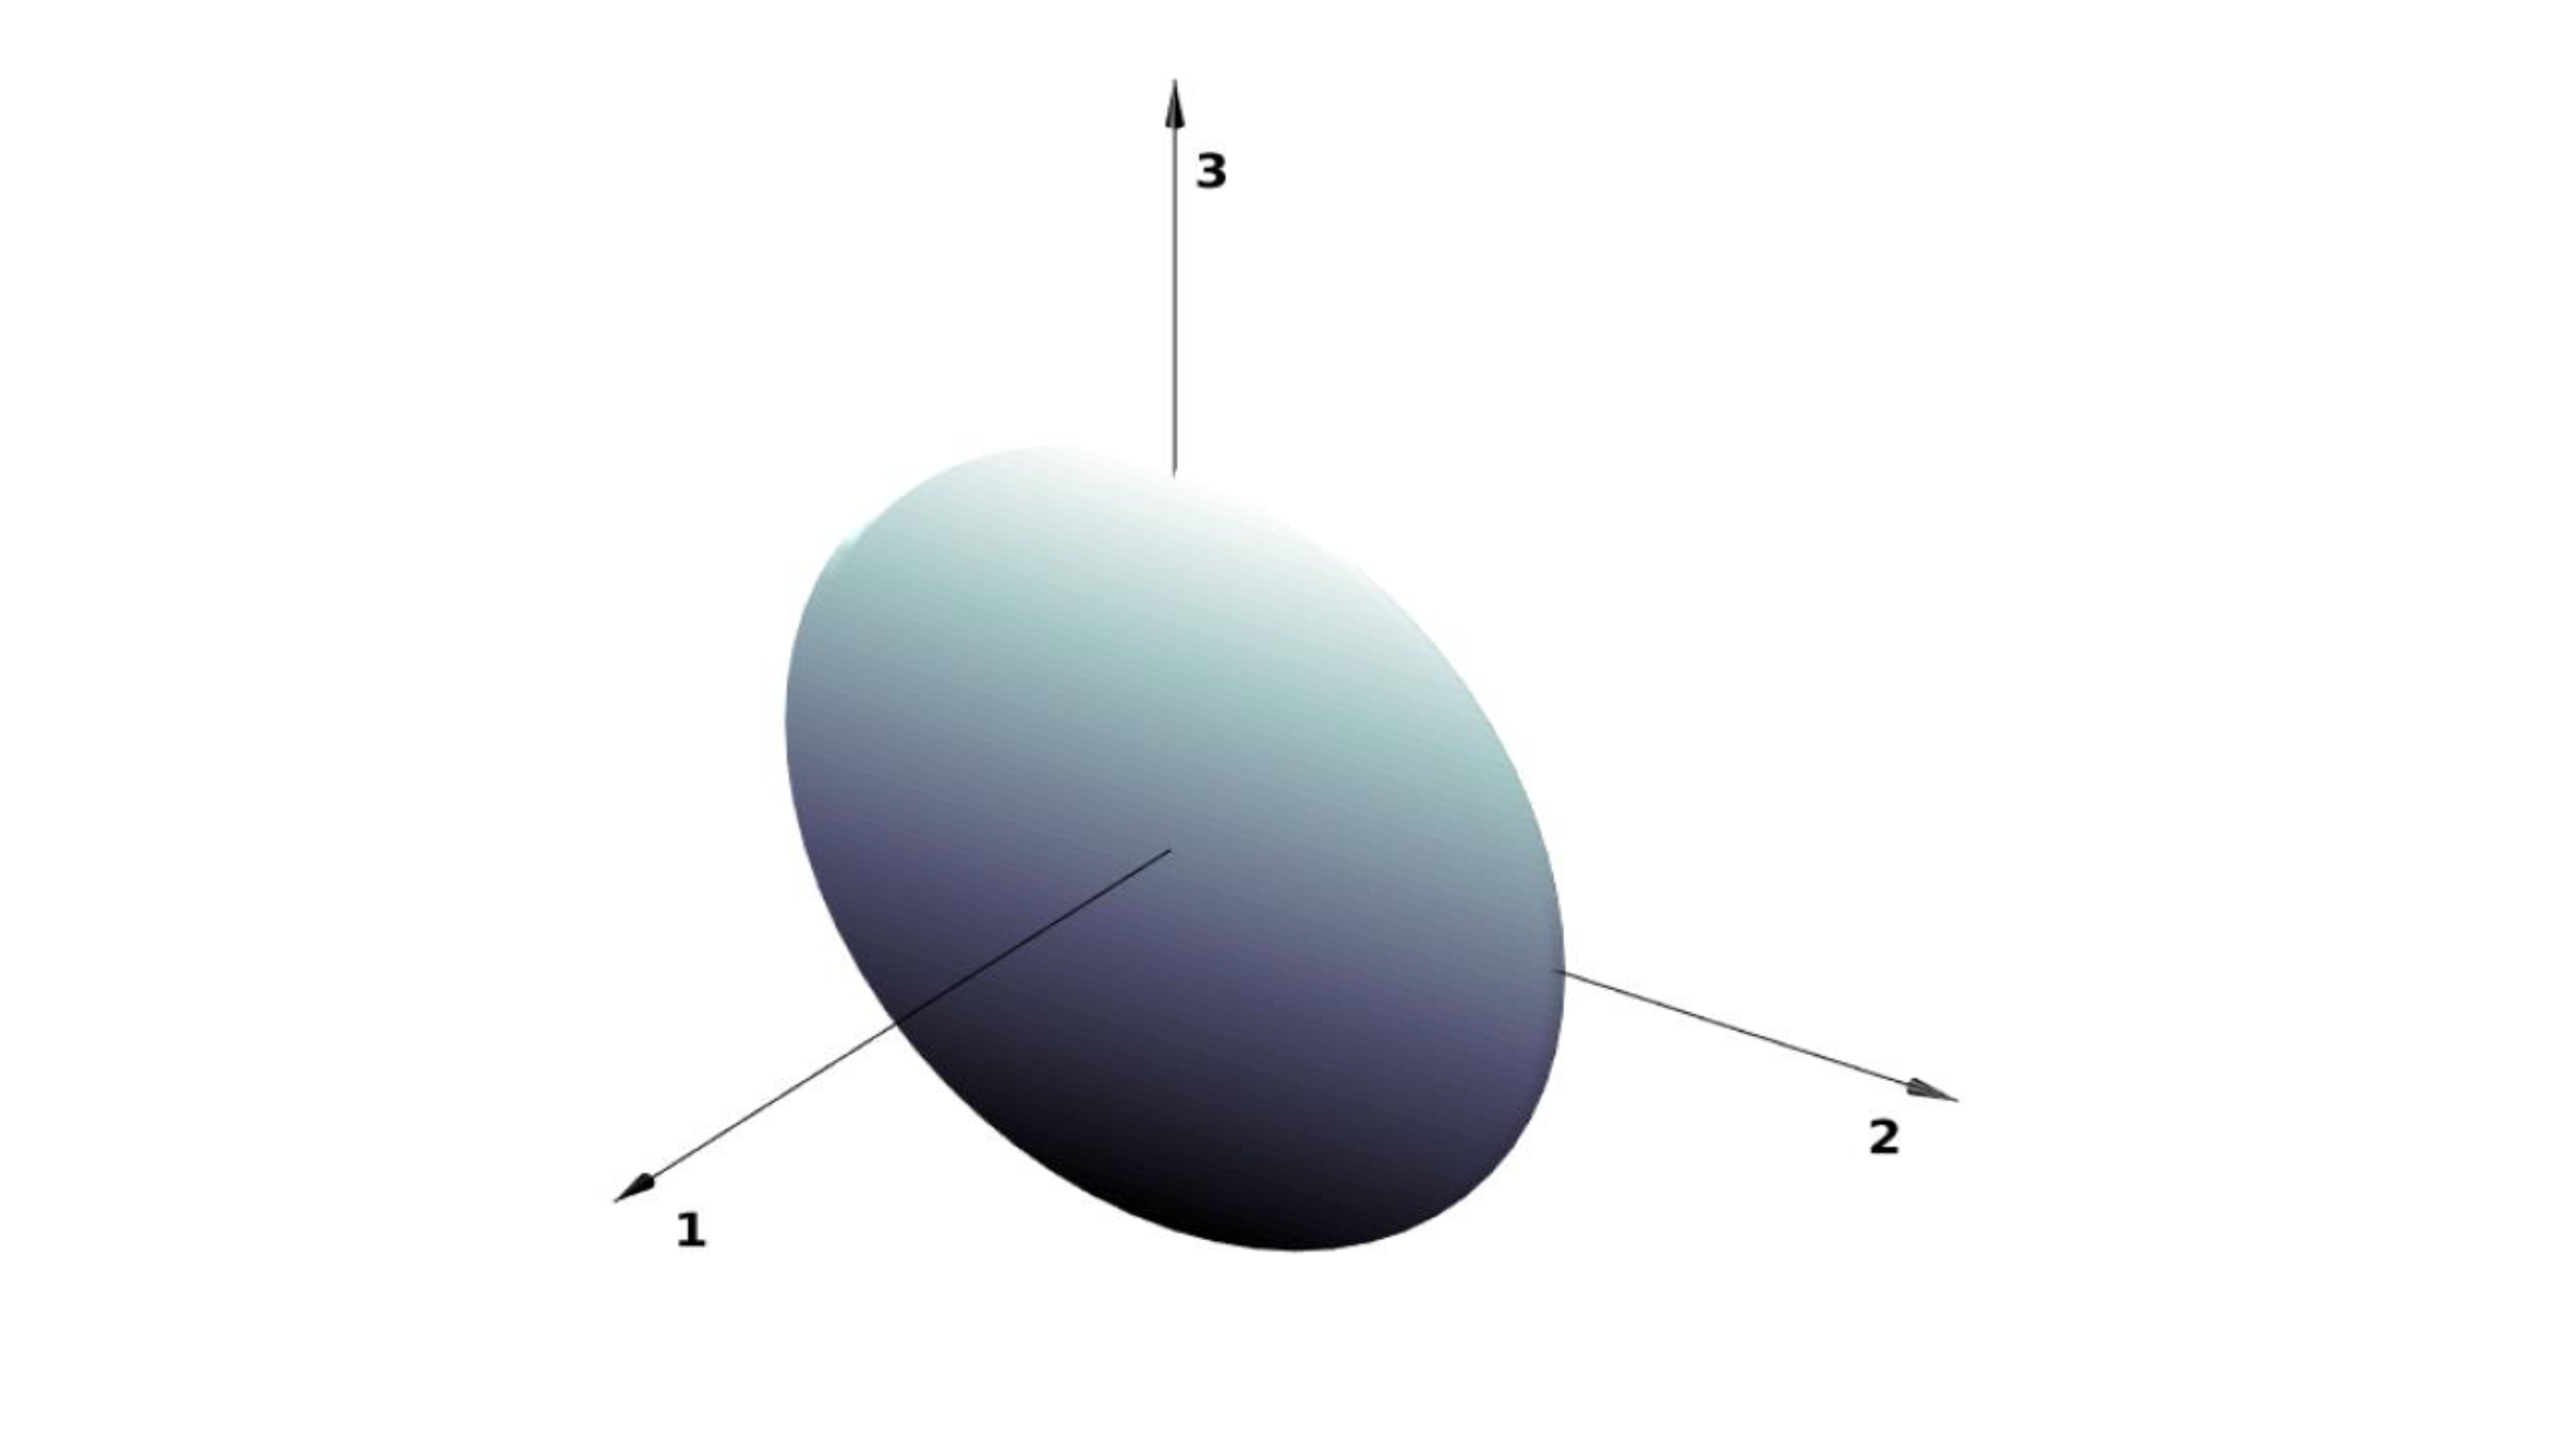
\includegraphics[trim=230 20 230 30, clip,             width=000.24\textwidth]{images/2c_min.png} 
        \label{fig:2c_min}
    }
    \end{subfigure}
    \hspace{10pt}
    \begin{subfigure}[$3C$ isotropic turbulence state.]{
        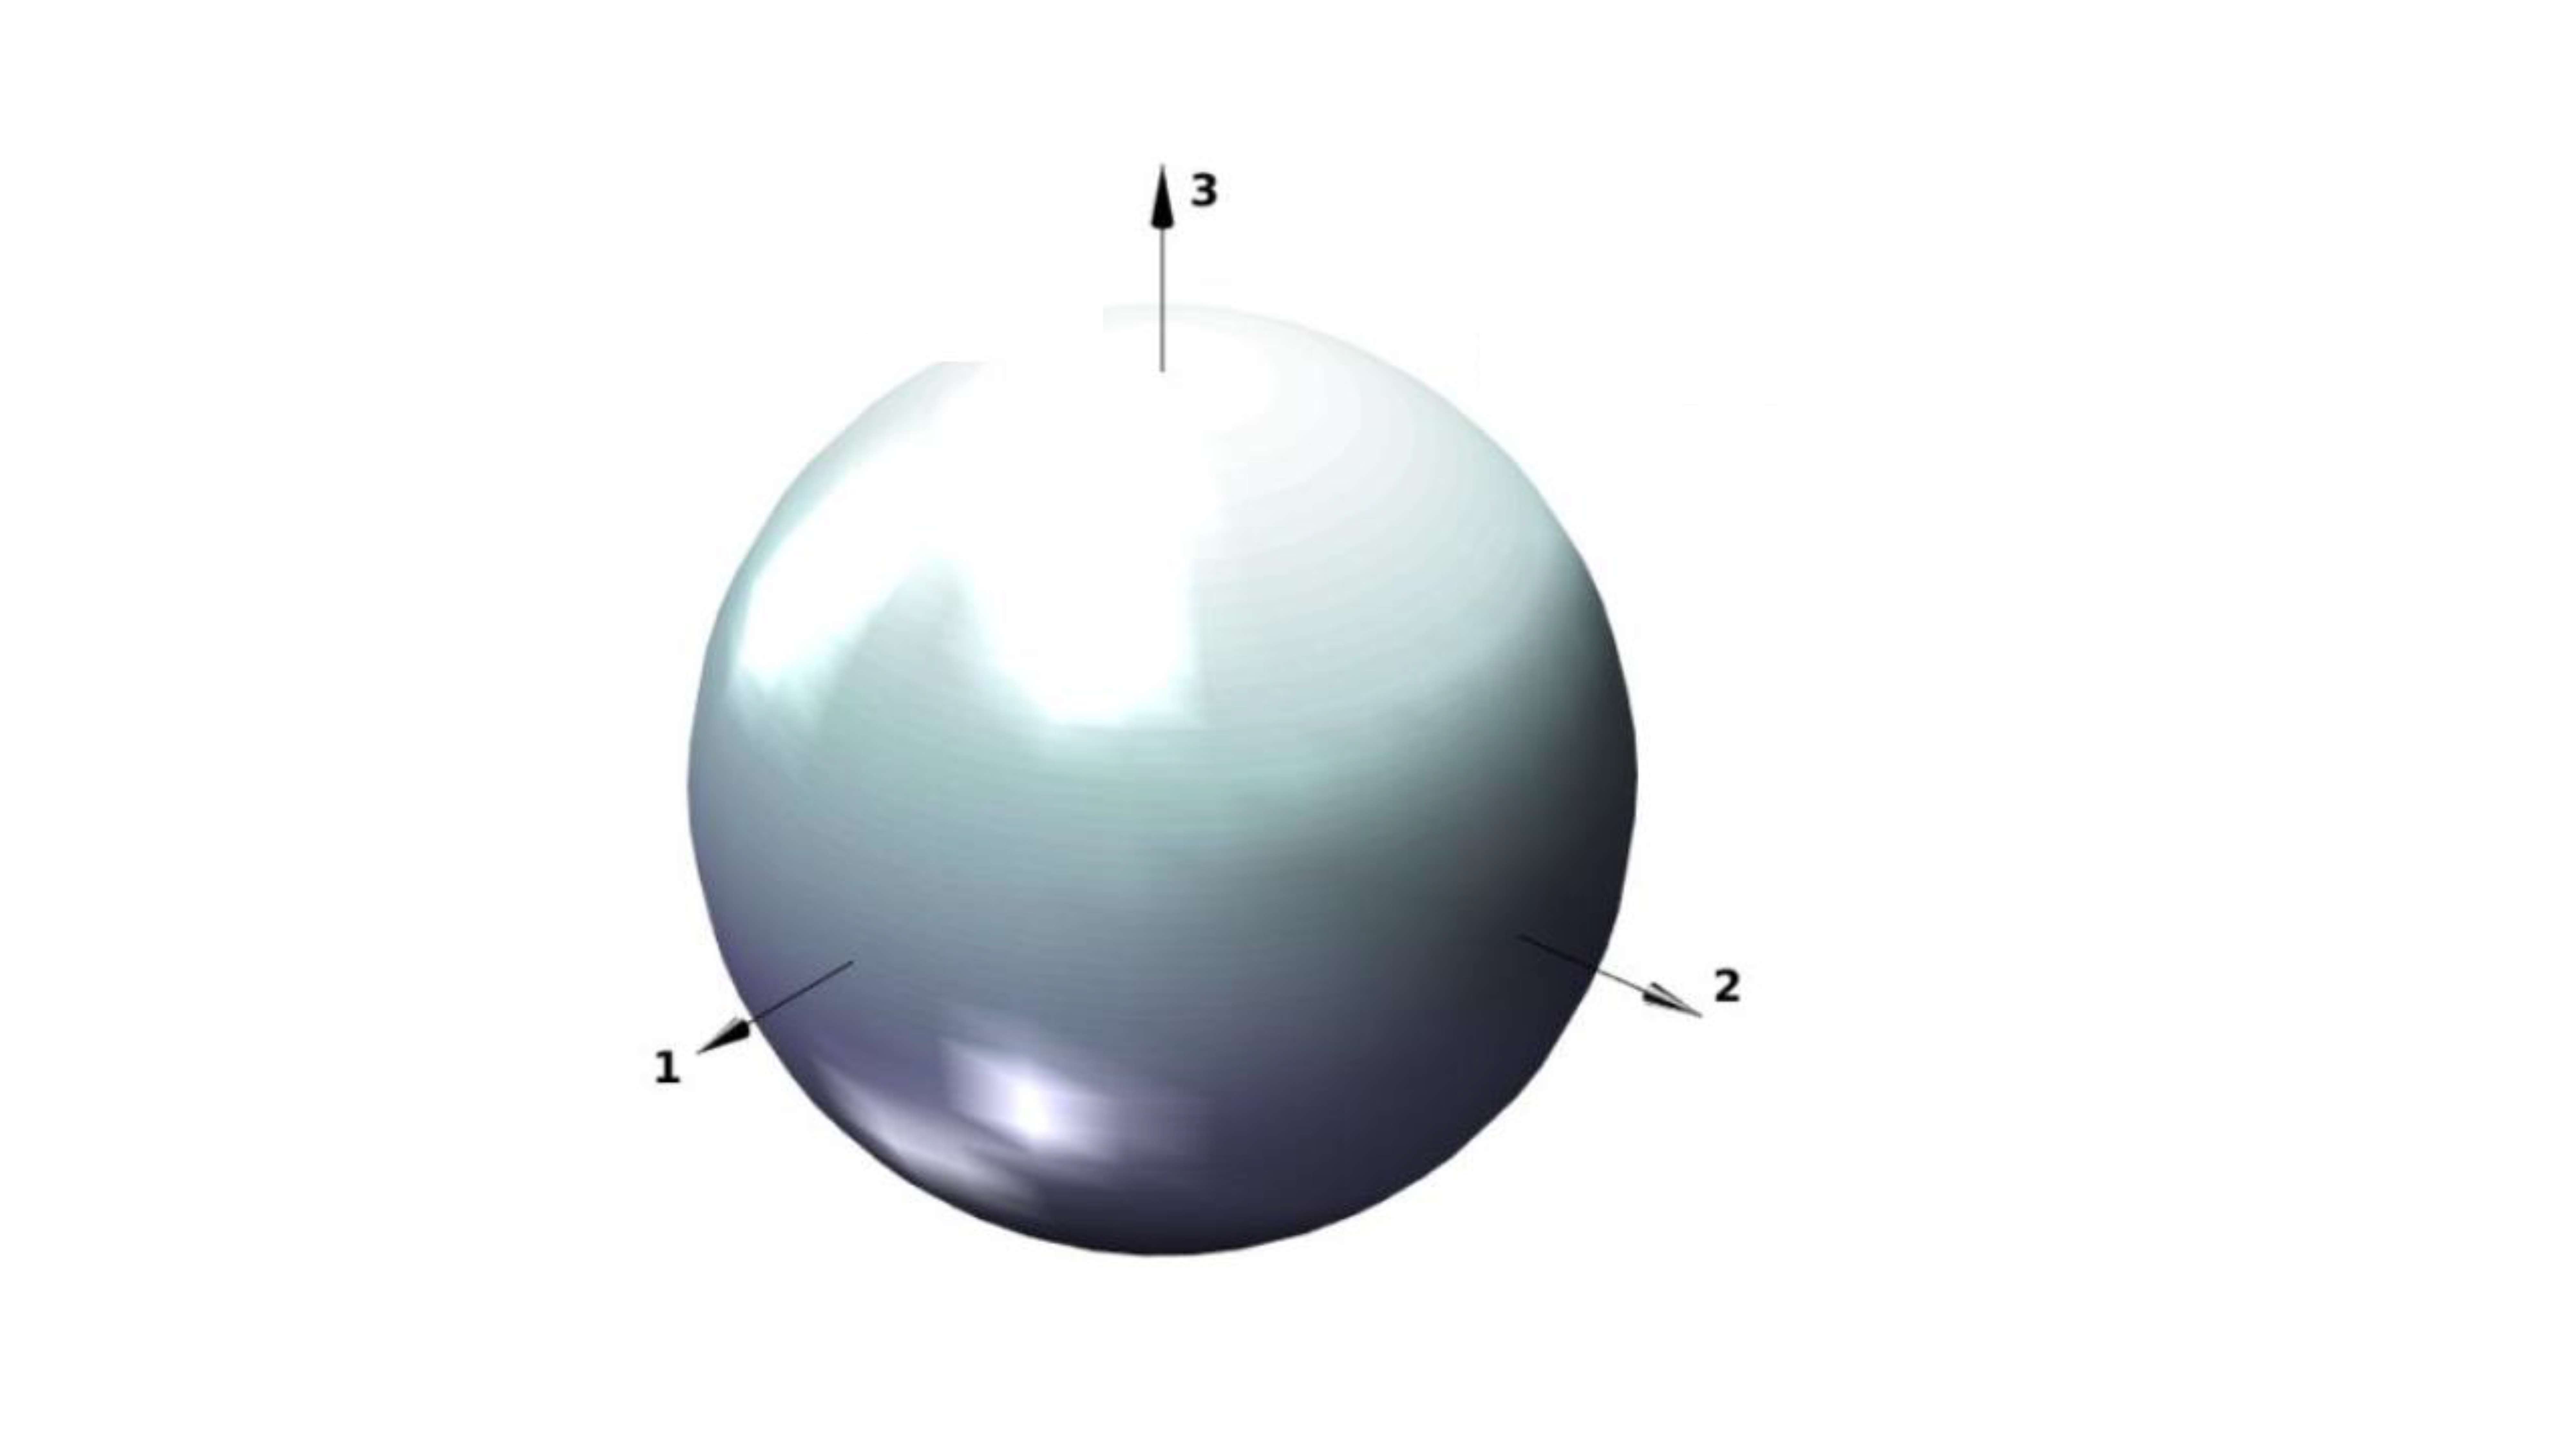
\includegraphics[trim=210 40 280 50, clip,             width=000.24\textwidth]{images/3c.png} 
        \label{fig:3c}
    }
    \end{subfigure}
    
    \begin{subfigure}[$1C$ state with $v_{max}$ eigenvector alignment.]{
        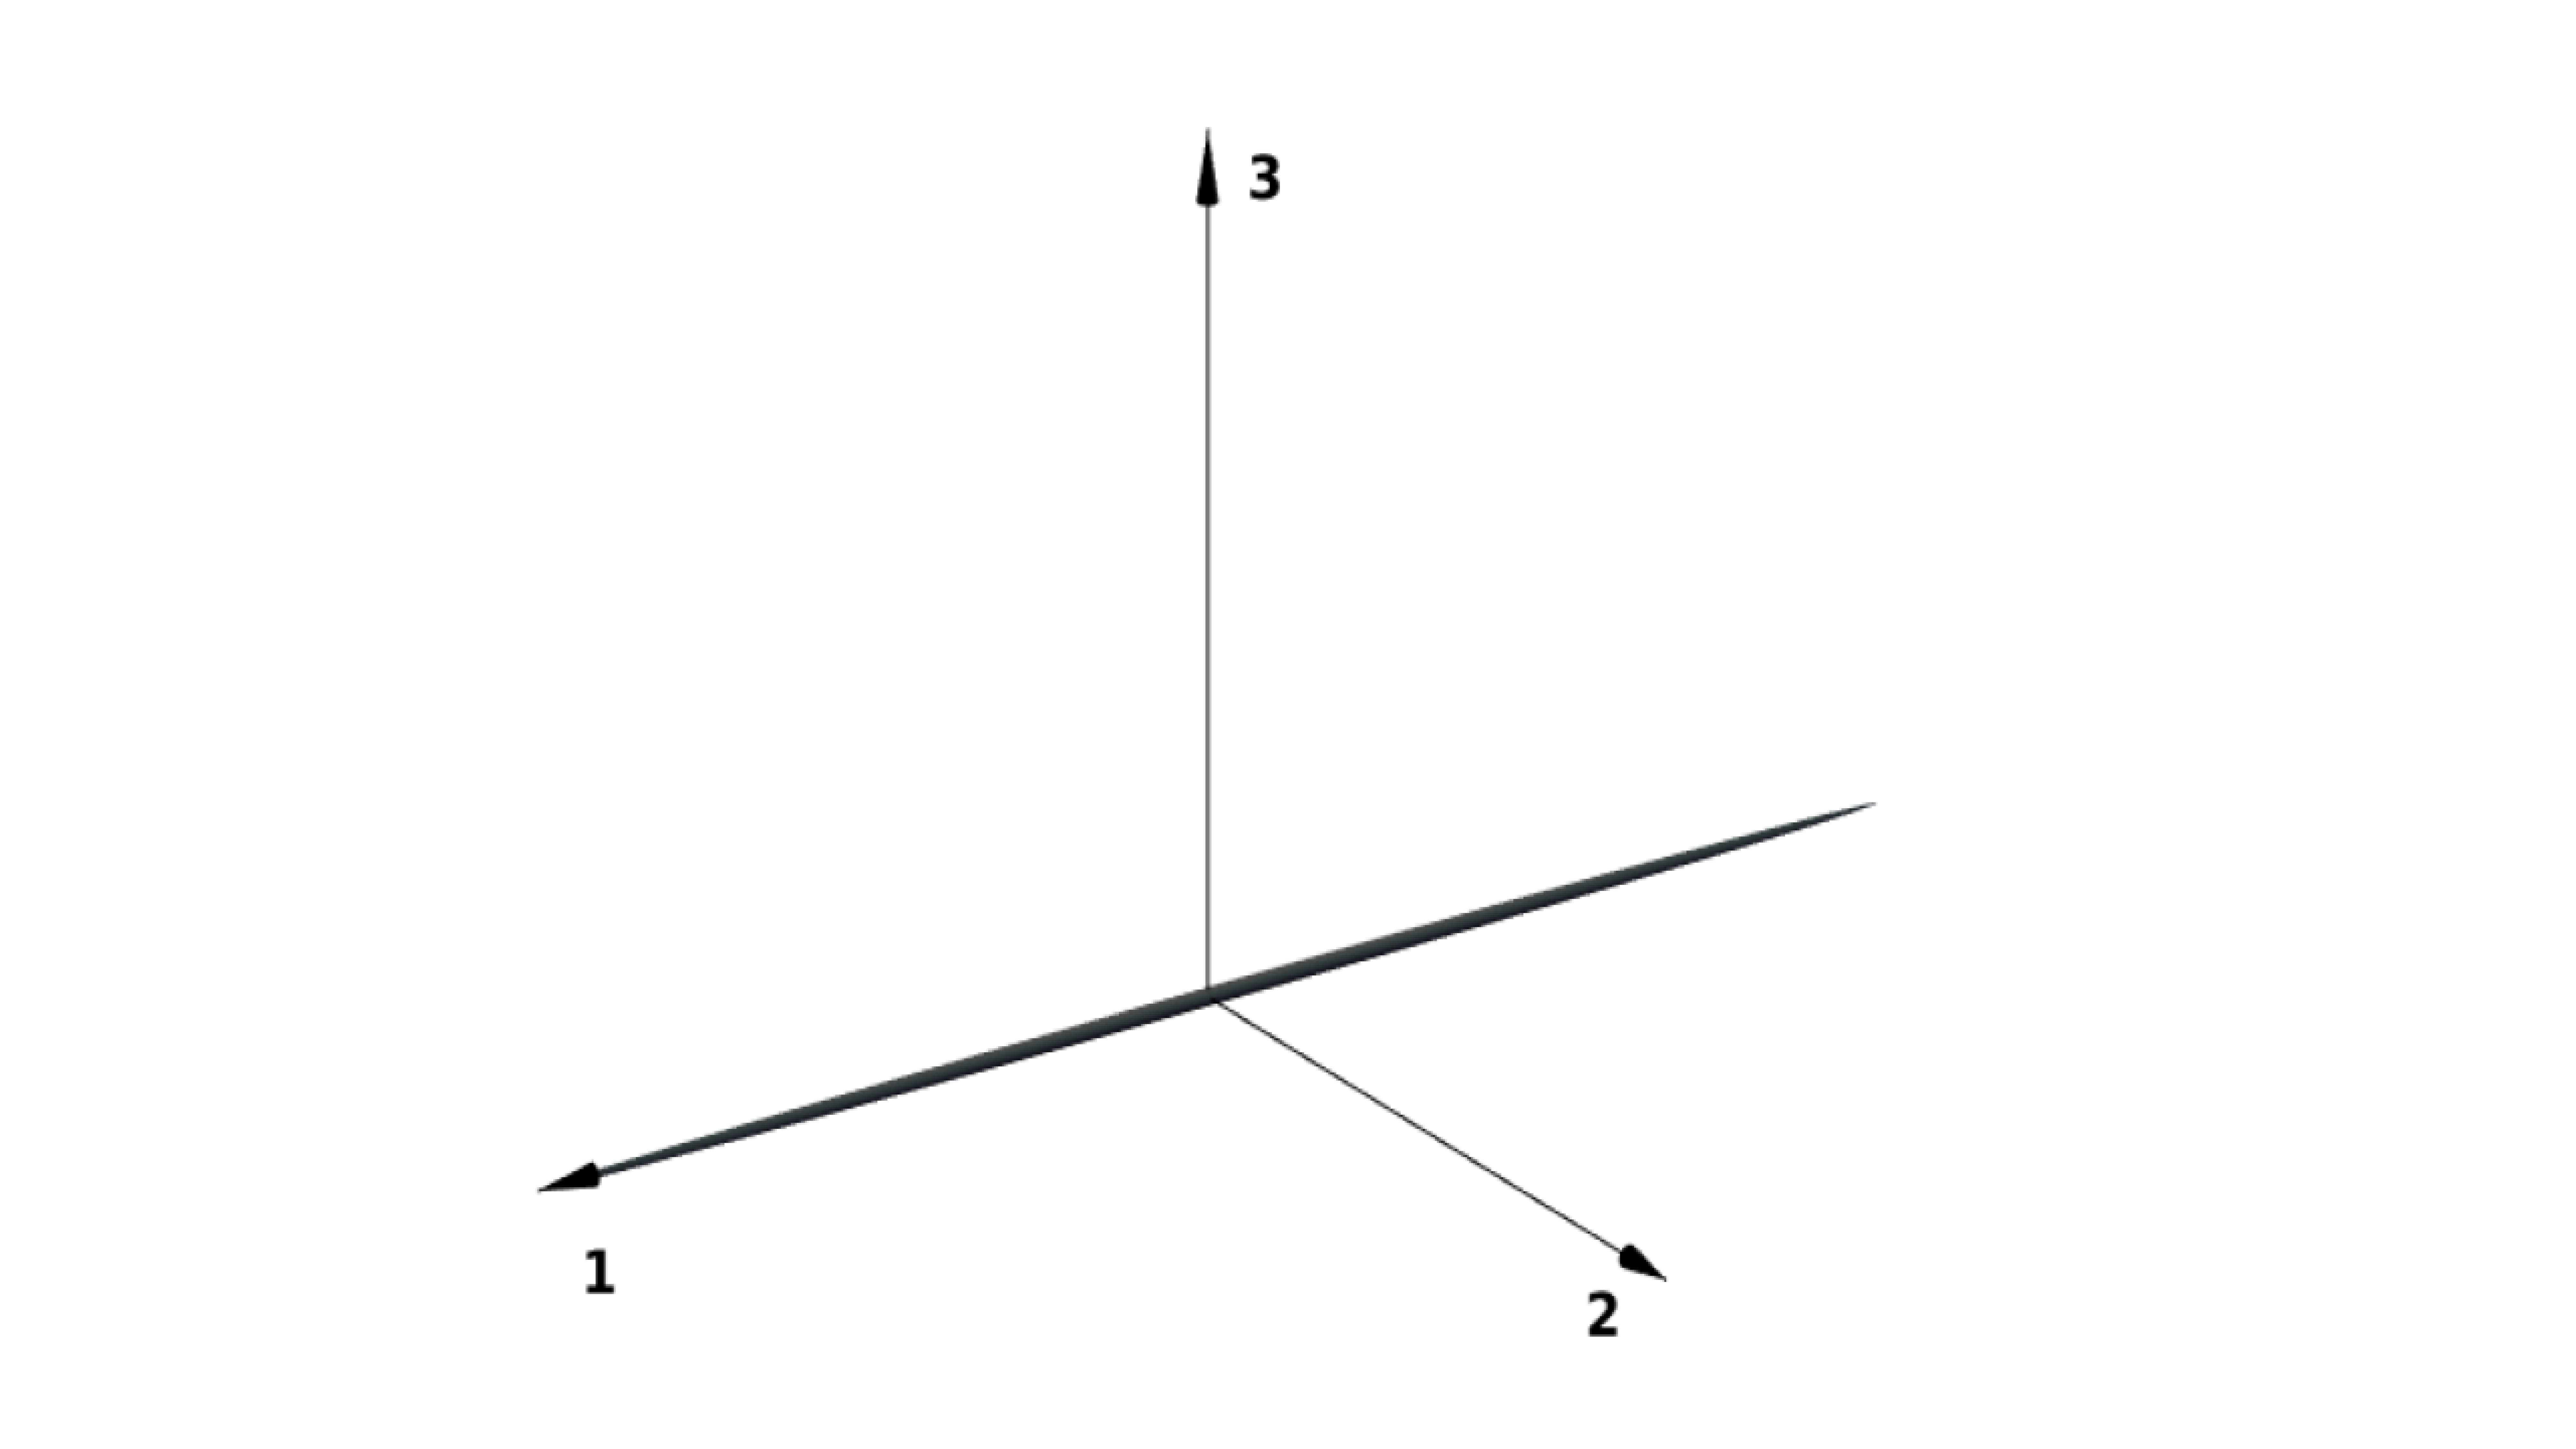
\includegraphics[trim=200 40 300 50, clip, width=0.24\textwidth]{images/1c_max.png}
        \label{fig:1c_max}
    }
    \end{subfigure}
    \hspace{10pt}
    \begin{subfigure}[$1C$ state with $v_{min}$ eigenvector alignment.]{
        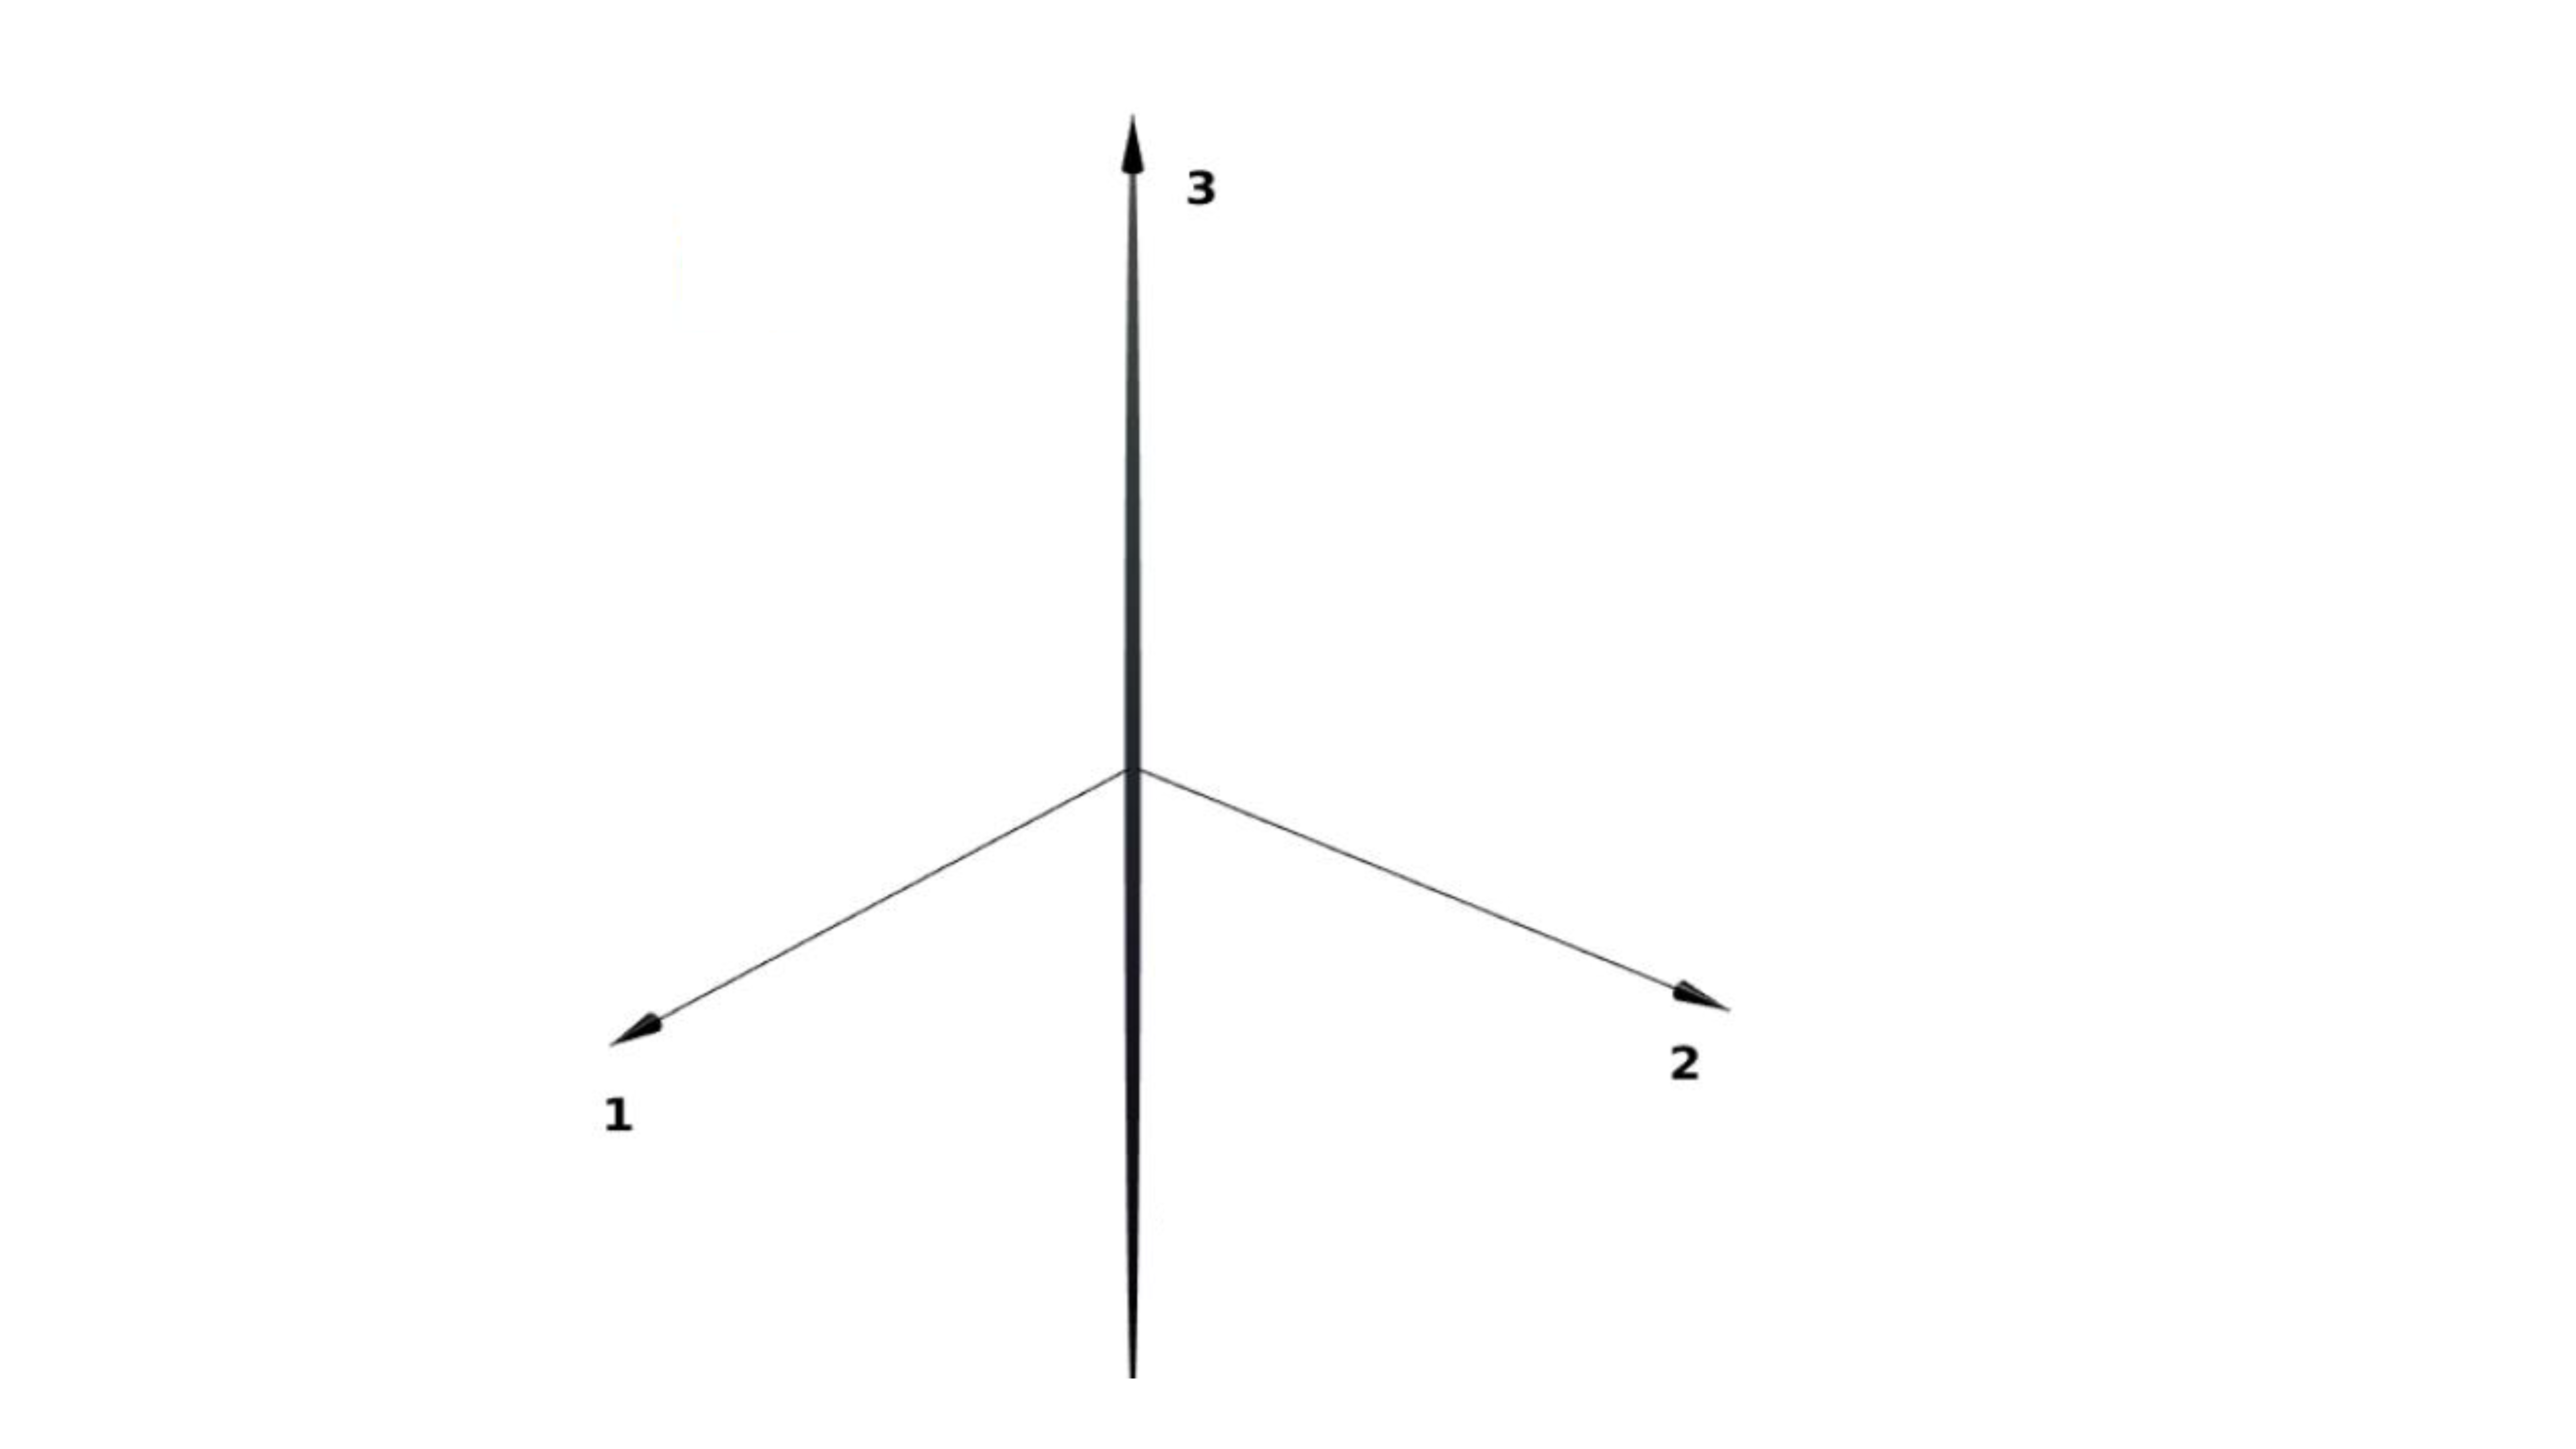
\includegraphics[trim=220 40 300 50, clip,             width=000.24\textwidth]{images/1c_min.png}
        \label{fig:1c_min}
    }
    \end{subfigure}
    \caption{Graphical visualization of each eigenspace perturbation as Reynolds stress ellipsoids. \label{fig:all_perts}}
\end{figure}

It is important to note that this methodology provides no probability distribution information for the QoIs within these interval bounds and assuming any particular distribution would be inconsistent with the methodology. From Section \ref{sec:mf_modeling}, the multi-fidelity GP requires data to be jointly normally distributed. Consequently, for the purpose of using these interval bounds in the multi-fidelity GP framework, a Gaussian distribution of the QoIs within the bound is assumed. The QoI is given by $y \sim \mathcal{N}(\mu,\sigma^2)$ where $\mu$ is the center of the bound, and $\sigma^2$ is calculated such that $95\%$ of the interval bound predicted by the RANS UQ methodology lies at $2\sigma$ from the mean, $\mu$.
